\documentclass[conference]{IEEEtran}
\IEEEoverridecommandlockouts
\usepackage{cite}
\usepackage{amsmath,amssymb}
\usepackage{graphicx}
\usepackage{booktabs}
\usepackage{array}
\usepackage{tikz}
\usetikzlibrary{arrows.meta,positioning}
\usepackage{pgfplots}
\pgfplotsset{compat=1.18}
\usepackage{microtype}
\usepackage{xurl}
\usepackage[hidelinks]{hyperref}
\urlstyle{same}

\newcommand{\Dr}{\emph{D.~radiodurans}}
\newcommand{\gene}[1]{\textit{#1}}

\begin{document}

\title{Network-Based Search for Functional Analogues of \emph{Deinococcus radiodurans} Stress
Defences in Humans: Oxidative Stress and DNA Repair}

\author{\IEEEauthorblockN{Ananthapadmanabhan}
\and
\IEEEauthorblockN{Pietro Hiram Guzzi}}

\maketitle

\begin{abstract}
\Dr\ survives doses of ionising radiation and desiccation that kill human cells, yet many of its
protective proteins have no human ortholog. We asked whether protein-network analysis can point to
human proteins that perform analogous functions without shared ancestry. We built STRING v12.5
functional-association networks (combined score $\geq 0.7$) of the Gene Ontology--defined
oxidative-stress and DNA-repair proteins of both species. We characterised their topology and
Louvain modules, aligned them with IsoRank against degree-preserving null models, and ranked every
cross-species protein pair with a transparent score that combines catalytic activity, GO and KEGG
annotation, experimental literature, mutant phenotypes, network context and graded homology.
Topology alone showed no conservation beyond degree-matched random graphs. Homology-anchored
alignment of the DNA-repair networks exceeded the null ($p = 0.01$--$0.02$), which partly reflects
STRING's transfer of evidence between orthologs. The ranking recovered known orthologs and proposed
candidate analogues, most clearly Mn/Fe versus Cu/Zn superoxide dismutases and Fpg/MutM versus
HhH-GPD DNA glycosylases. Curated mutant studies contradicted simple protective roles for
\gene{sodA} and \gene{lexA}, and no experimentally determined physical interactions exist for the
bacterial proteins in IntAct, BioGRID or MINT. All results are computational candidates; we propose
specific complementation experiments to test them.
\end{abstract}

\begin{IEEEkeywords}
protein networks, network alignment, functional analogy, \emph{Deinococcus radiodurans},
oxidative stress, DNA repair, reproducibility
\end{IEEEkeywords}

\section{Introduction}

The bacterium \Dr\ recovers from acute ionising-radiation doses above 10\,kGy and grows under
chronic irradiation \cite{daly2004}. Two explanations dominate. First, efficient DNA repair
reassembles its shattered genome. Second, high intracellular Mn(II) relative to iron protects
proteins from oxidative damage, so that the repair machinery itself survives
\cite{daly2004,daly2007,daly2009,slade2011}. Both are attractive starting points for understanding,
and perhaps strengthening, human resistance to oxidative and genotoxic stress.

Transferring this knowledge to humans is hard because many Deinococcus factors, such as DdrA,
DdrB and PprA, have no human ortholog. Sequence-based orthology inference \cite{orthofinder}
therefore misses exactly the proteins that make the organism unusual. Network-level comparison
offers an alternative: proteins can occupy equivalent positions in their interaction networks
without sharing ancestry. Network alignment methods such as IsoRank \cite{isorank} and MAGNA++
\cite{magna} formalise this idea, and the trade-offs between local and global alignment are well
documented \cite{guzzi2018}.

Three obstacles limit such comparisons. Bacterial interaction data are sparse and biased towards
well-studied proteins. Functional associations are easily mistaken for physical interactions. And
there is no ground truth for cross-species functional analogy, so accuracy claims cannot be made.
We therefore designed the analysis to report what the data can and cannot support. Our
contributions are:
\begin{itemize}
  \item a reproducible pipeline that builds and quality-controls cross-species networks from
    public resources, with cached and checksummed inputs and byte-identical reruns;
  \item an evidence-graded classification that separates orthologs, homologs, distant homologs
    (shared fold only) and candidate analogues, and never treats missing evidence as negative;
  \item network alignment tested against degree-preserving null models rather than random
    mappings alone;
  \item an application to two processes, oxidative-stress defence and DNA repair, including
    negative results and literature findings that contradict simple interpretations.
\end{itemize}

\section{Materials and Methods}

Fig.~\ref{fig:pipeline} summarises the workflow. All parameters are stored in versioned
configuration files and copied into each run's manifest.

\begin{figure}[t]
\centering
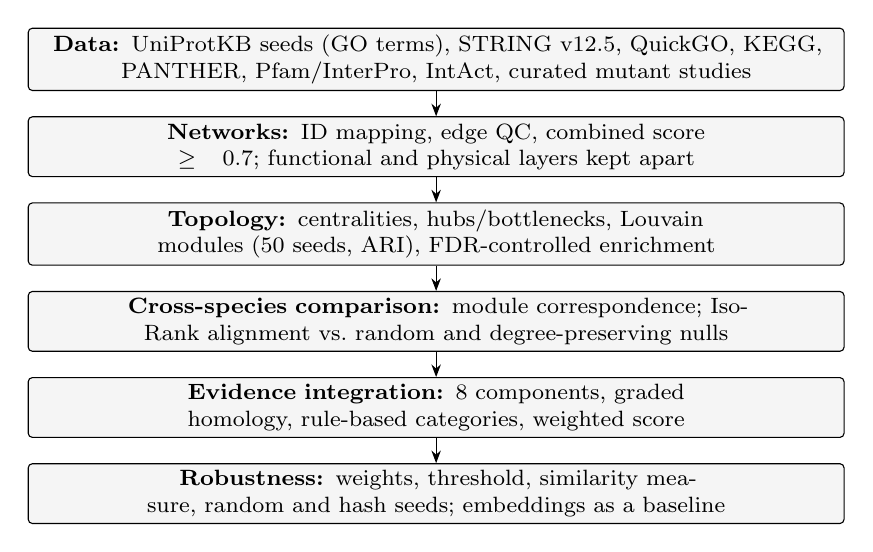
\begin{tikzpicture}[
  node distance=3.2mm,
  box/.style={draw, rounded corners=1.5pt, align=center, font=\footnotesize,
              text width=0.84\columnwidth, inner sep=2.5pt, fill=black!4},
  arr/.style={-{Stealth[length=1.6mm]}, thin}]
\node[box] (data) {\textbf{Data:} UniProtKB seeds (GO terms), STRING v12.5, QuickGO, KEGG,\\
  PANTHER, Pfam/InterPro, IntAct, curated mutant studies};
\node[box, below=of data] (net) {\textbf{Networks:} ID mapping, edge QC, combined score $\geq 0.7$;
  functional and physical layers kept apart};
\node[box, below=of net] (topo) {\textbf{Topology:} centralities, hubs/bottlenecks,
  Louvain modules (50 seeds, ARI), FDR-controlled enrichment};
\node[box, below=of topo] (cmp) {\textbf{Cross-species comparison:} module correspondence;
  IsoRank alignment vs.\ random and degree-preserving nulls};
\node[box, below=of cmp] (rank) {\textbf{Evidence integration:} 8 components, graded homology,
  rule-based categories, weighted score};
\node[box, below=of rank] (rob) {\textbf{Robustness:} weights, threshold, similarity measure,
  random and hash seeds; embeddings as a baseline};
\foreach \src/\dst in {data/net, net/topo, topo/cmp, cmp/rank, rank/rob} \draw[arr] (\src) -- (\dst);
\end{tikzpicture}
\caption{Analysis workflow. Every step reads cached, checksummed inputs and writes a manifest.}
\label{fig:pipeline}
\end{figure}

\subsection{Seed proteins and networks}

Seed proteins are UniProtKB \cite{uniprot2025} entries annotated with the relevant Gene Ontology
\cite{go2023} terms, including descendant terms: GO:0006979 (response to oxidative stress),
GO:0098869 (cellular oxidant detoxification) and GO:0016209 (antioxidant activity) for oxidative
stress, and GO:0006281 (DNA repair) for DNA repair. For human, only reviewed (Swiss-Prot) entries
are used; for \Dr, which has few reviewed entries, all entries are used. Seeds are mapped to
STRING v12.5 \cite{string2025}, which resolves \Dr\ (NCBI 1299) to strain R1 (taxon 243230).
Unmapped seeds are reported and never substituted.

Networks are retrieved from STRING at combined score $\geq 0.4$ and thresholded at $0.7$ for
analysis, so other thresholds can be re-applied offline. Edges pass ordered quality checks
(identifier validity, species, self-loops, score range, duplicates), and every excluded record is
listed with its reason. STRING edges are functional associations. Edges also present in STRING's
physical subnetwork are flagged, and physical interactions are checked separately in IntAct
\cite{intact2022} through PSICQUIC \cite{psicquic}; this layer is reported but not used for ranking.

\subsection{Annotation and graded homology}

Each protein is annotated with GO terms and evidence codes (QuickGO \cite{quickgo}; NOT
qualifiers are kept as contradicting evidence), KEGG pathways and KEGG Orthology (KO) groups
\cite{kegg2025}, EC numbers, PANTHER families \cite{panther2022}, and Pfam and InterPro
signatures \cite{interpro2025}. Homology between a bacterial and a human protein is graded by the
first tier that applies: reciprocal best hit in STRING's Smith--Waterman searches (bitscore
$\geq 50$; score 1.0), shared KO group (0.9), shared PANTHER family (0.8), one-way best hit (0.6),
shared Pfam domain (0.5), shared InterPro entry (0.4), and a shared \emph{common-fold} signature
only (0.2). Signatures carried by more than 5\,\% of all network proteins (for example the
thioredoxin fold or the P-loop NTPase) define the common-fold tier. They are kept rather than
discarded, because discarding them turned true homologs into false analogues. Since every protein
is searched, ``no homology detected'' is an observation, not a missing value.

\subsection{Topology and modules}

For each network we compute degree, betweenness and closeness (edge length $1/\text{score}$),
clustering, PageRank and k-core, with percentiles taken within species over connected nodes.
Hubs and bottlenecks are nodes in the top 20\,\% of degree and betweenness \cite{yu2007}.
Modules are found with weighted Louvain \cite{louvain} at resolution 1.0 over 50 random seeds. The
reported partition is the medoid run, and stability is the mean pairwise adjusted Rand index
(ARI) \cite{ari}. Module enrichment uses a one-sided hypergeometric test against the species'
seed network as background, with Benjamini--Hochberg correction across all tests \cite{bh}
(FDR $\leq 0.05$). A genome background would trivially enrich the GO terms used to select the
seeds. Because the human networks are much larger, they are also subsampled to the bacterial node
count (1,000 samples) to put bacterial statistics in context.

\subsection{Cross-species comparison}

\emph{Module correspondence} compares the core terms (carried by at least half the members) of
each pair of non-singleton modules. \emph{Network alignment} uses IsoRank \cite{isorank}, which
computes a node-similarity matrix $R$ from the fixed point
\begin{equation}
R = \alpha\, A R + (1 - \alpha)\, E,
\end{equation}
where $A$ is the normalised product of the two adjacency matrices and $E$ is a homology prior built
from STRING bitscores. $\alpha = 1$ uses topology only. A greedy one-to-one matching then gives the
alignment, scored by the number of conserved bacterial edges. Beating random one-to-one mappings
(1,000 samples) only shows that the optimiser works. The decisive test aligns
degree-preserving rewired copies of the bacterial network \cite{maslov2002} in the same way
(100 samples; 200 for the small coverage variant below) and asks whether the real network aligns
better.

To test whether conclusions depend on coverage, a \emph{KO-projected} bacterial network adds every
\Dr\ gene whose KO group is carried by a human seed. It is used only for alignment, never for
ranking, because it is defined by orthology.

\subsection{Evidence integration and ranking}

Every bacterial--human protein pair $p$ is scored on eight components $s_i(p) \in [0,1]$:
shared EC number (complete number 1.0, same sub-subclass 0.5), GO similarity, KEGG pathway
similarity, experimental literature, perturbation (mutant) evidence, module similarity, network-role
similarity and homology. Set similarities use information-content-weighted Ochiai similarity,
\begin{equation}
\mathrm{sim}(A,B) = \frac{\sum_{t \in A \cap B} \mathrm{IC}(t)}
{\sqrt{\sum_{t \in A} \mathrm{IC}(t) \sum_{t \in B} \mathrm{IC}(t)}},
\end{equation}
where $\mathrm{IC}(t) = -\ln p(t)$ is the information content of term $t$ in the annotations of
both networks. Ochiai is used because annotation depth differs greatly between the species; simGIC \cite{pesquita2008} and a
min-normalised variant are run as sensitivity analyses. The score of a pair is a weighted mean over
the components $\mathcal{A}(p)$ that are available for it,
\begin{equation}
S(p) = \frac{\sum_{i \in \mathcal{A}(p)} w_i\, s_i(p)}{\sum_{i \in \mathcal{A}(p)} w_i},
\qquad C(p) = \sum_{i \in \mathcal{A}(p)} w_i ,
\end{equation}
so missing evidence never lowers a score. The weights are 0.15 for EC, GO, pathway and literature
and 0.10 for perturbation, module, role and homology. Pairs with evidence coverage $C(p) < 0.45$
are listed but not ranked.

Perturbation evidence combines GO mutant codes with a literature-curated table of \Dr\ mutant and
biochemical studies (8 findings for 5 oxidative-stress proteins and 13 for 7 DNA-repair proteins),
each checked against its PubMed abstract. Findings that \emph{contradict} a protective role are
kept: a protein scores 1 if all its evidence supports the role, 0.5 if mixed and 0 if only
contradicting.

Independently of the score, fixed rules assign each pair one category: \emph{ortholog} (reciprocal
best hit, or shared KO), \emph{homolog} (PANTHER, one-way hit, Pfam or InterPro tier),
\emph{distant homolog} (common fold only), \emph{candidate analogue} (no homology, shared EC
sub-subclass, and independent pathway, GO or experimental support), \emph{shared function}
(no homology, EC or GO similarity only), \emph{similar pathway role} (shared KEGG pathways only),
and \emph{speculative} or \emph{unsupported}.

\subsection{Robustness, embeddings and evaluation}

We perturbed the weights (500 Dirichlet samples, concentration 50), removed each component in
turn, varied the similarity measure and the STRING threshold (0.4--0.9), and repeated runs with
different random seeds and Python hash seeds. As a graph-learning baseline, NetMF embeddings
\cite{netmf} (16 dimensions, window 5) were evaluated by within-species link prediction on held-out
edges (5 splits of 10\,\%) against common-neighbour, Jaccard and Adamic--Adar \cite{adamic2003}
scores. Embeddings were not compared across species, because independently factorised graphs share
no coordinate system. As there is no ground truth for analogy, we report only a proxy: how well
each component separates known ortholog pairs from other pairs, with an AUC treated as evaluable
only for at least 10 positive pairs.

\subsection{Implementation}

The pipeline is written in Python with NetworkX \cite{networkx} and Pandas. All API responses are
cached immutably with SHA-256 checksums; inputs are re-verified before each analysis, every run
writes a manifest, and result tables are byte-identical across reruns and hash seeds. It runs with
one command and has 88 automated tests with mocked APIs.

\section{Results}

\subsection{Networks and coverage}

Table~\ref{tab:networks} summarises the four networks. The oxidative-stress network of \Dr\ is
small: 16 proteins and 11 edges, with 9 proteins isolated. This reflects the size of the GO-defined
seed set rather than poor connectivity. Random 16-protein subsets of the human seeds have 3.5 edges
on average (95th percentile 9), and the bacterial set has more edges than 97.7\,\% of them.
Projecting via KO adds little: of 345 human seed KO groups, only 16 \Dr\ genes match, giving a
network of 27 proteins and 16 edges. The DNA-repair networks are much better balanced, with 52
bacterial and 426 human proteins. The bacterial DNA-repair set is also more connected than random
human subsets of equal size (119 edges versus a mean of 77, above 95.3\,\% of subsets).

\begin{table}[t]
\centering
\caption{Networks at STRING combined score $\geq 0.7$}
\label{tab:networks}
\footnotesize
\setlength{\tabcolsep}{4pt}
\begin{tabular}{lrrrr}
\toprule
 & \multicolumn{2}{c}{Oxidative stress} & \multicolumn{2}{c}{DNA repair} \\
\cmidrule(lr){2-3}\cmidrule(lr){4-5}
 & D.r. & H.s. & D.r. & H.s. \\
\midrule
seeds / mapped & 16 / 16 & 385 / 382 & 56 / 52 & 432 / 426 \\
edges & 11 & 2,210 & 119 & 5,285 \\
isolated proteins & 9 & 70 & 11 & 23 \\
largest component & 5 & 295 & 41 & 400 \\
edges in IntAct & 0 & 275 & 0 & 431 \\
\bottomrule
\end{tabular}\\[3pt]
D.r., \emph{D.~radiodurans}; H.s., \emph{H.~sapiens}.
\end{table}

\subsection{Modules}

Louvain modules of the human oxidative-stress network (mean ARI 0.74 across 50 seeds; modularity
0.54) include a 69-protein antioxidant and detoxification module (SOD1--3, CAT, PRDX1--6,
GPX2--8, TXNRD1--3, glutathione synthesis and transferases, NFE2L2/KEAP1), a proteasome module and a
mitochondrial inner-membrane module. The two non-trivial bacterial components, \{\gene{katA},
DRA0259, \gene{sodA}, \gene{sodC}, DRA0202\} and \{DR1208, DR1209\}, both match the human
antioxidant module best. Their only significant term, the KEGG map ``Peroxisome'', is an artefact
of ortholog-based map membership, because bacteria have no peroxisomes.

In DNA repair, all five non-singleton bacterial modules (mean ARI 0.76) are FDR-significant and
correspond to known pathways: base-excision repair; RecFOR recombination; nucleotide-excision
repair (UvrABC, Mfd); replication and mismatch repair; and a radiation-response module containing
RecA, LexA, DdrA, DdrB and PprA. The human network separates into Fanconi anaemia and D-loop
resolution, replication, base-excision, nucleotide-excision, translesion-synthesis and SMC5/6
modules. Module correspondence was, however, weakly discriminating: several bacterial modules
matched the human base-excision module best, because generic repair terms dominate the profiles.

\subsection{Network alignment}

Table~\ref{tab:alignment} shows the alignment tests. All alignments conserved more edges than
random mappings ($p = 1/1001$, the smallest value 1,000 samples can give), but this only confirms
that the optimiser works. Against degree-preserving rewired networks, oxidative-stress topology showed no conservation, either for
the seed network or for the KO-projected network. The only low $p$-value (0.02) came from the
KO-prior alignment of the projected network, which is not independent evidence (see below). For
DNA repair, topology alone was not significant either ($p = 0.08$), while homology-anchored alignment
exceeded the null ($p = 0.01$--$0.02$; KO-projected variant $p = 0.005$). With 100 rewired samples the
smallest attainable $p$ is $1/101 \approx 0.01$ (and $1/201$ with 200 samples), so these values
sit at the resolution limit of the test.

These $p$-values must be read with one caveat. STRING transfers association evidence between
orthologs of different organisms, so edge conservation between orthologous pairs is partly built
into the input scores. The DNA-repair result is therefore consistent with conserved pathway
structure but cannot demonstrate it.

\begin{table}[t]
\centering
\caption{IsoRank alignment against degree-preserving rewired nulls (empirical $p$; 100
samples, 200 for the KO-projected network)}
\label{tab:alignment}
\footnotesize
\setlength{\tabcolsep}{4pt}
\begin{tabular}{lrr}
\toprule
prior ($\alpha$) & conserved edges & $p$ \\
\midrule
\multicolumn{3}{l}{\emph{Oxidative stress, seed network (11 edges)}} \\
\quad none (1.0) & 9 & 0.10 \\
\quad homology (0.8) & 8 & 0.63 \\
\quad homology (0.5) & 7 & 0.88 \\
\addlinespace
\multicolumn{3}{l}{\emph{Oxidative stress, KO-projected network (16 edges)}} \\
\quad none (1.0) & 9 & 1.0 \\
\quad shared KO (0.8) & 13 & 0.02 \\
\addlinespace
\multicolumn{3}{l}{\emph{DNA repair, seed network (119 edges)}} \\
\quad none (1.0) & 114 & 0.08 \\
\quad homology (0.8) & 87 & 0.02 \\
\quad homology (0.5) & 89 & 0.01 \\
\bottomrule
\end{tabular}
\end{table}

\subsection{Candidate relationships}

All 6,112 oxidative-stress pairs and 22,152 DNA-repair pairs were scored; 4,329 and 20,020 had
enough evidence to be ranked. Fig.~\ref{fig:categories} shows the eligible pairs per category, and
Table~\ref{tab:pairs} lists representative pairs.

\begin{figure}[t]
\centering
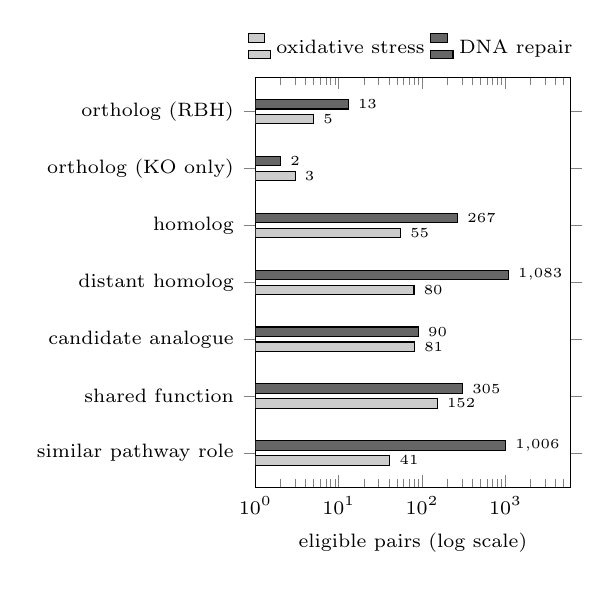
\begin{tikzpicture}
\begin{axis}[
  xbar, xmode=log, log origin=infty,
  scale only axis, width=4.0cm, height=5.2cm,
  bar width=3.4pt,
  xmin=1, xmax=6000,
  xlabel={eligible pairs (log scale)},
  ytick={1,...,7},
  yticklabels={ortholog (RBH), ortholog (KO only), homolog, distant homolog,
               candidate analogue, shared function, similar pathway role},
  y dir=reverse, enlarge y limits=0.1,
  tick label style={font=\scriptsize}, label style={font=\scriptsize},
  legend style={font=\scriptsize, at={(0.5,1.02)}, anchor=south, legend columns=2,
                draw=none},
  point meta=rawx,
  nodes near coords,
  every node near coord/.append style={font=\tiny, anchor=west}]
\addplot[draw=black, fill=black!20] coordinates {
  (5,1) (3,2) (55,3) (80,4) (81,5) (152,6) (41,7)};
\addplot[draw=black, fill=black!60] coordinates {
  (13,1) (2,2) (267,3) (1083,4) (90,5) (305,6) (1006,7)};
\legend{oxidative stress, DNA repair}
\end{axis}
\end{tikzpicture}
\caption{Eligible protein pairs per evidence category. Speculative and unsupported pairs are not
shown.}
\label{fig:categories}
\end{figure}

\begin{table*}[t]
\centering
\caption{Representative pairs. Rank among eligible pairs, with the 5--95\,\% interval under 500
weight perturbations.}
\label{tab:pairs}
\footnotesize
\begin{tabular}{llll>{\raggedright\arraybackslash}p{6.2cm}r}
\toprule
process & \Dr & human & category & basis & rank [5--95\,\%] \\
\midrule
Oxidative & \gene{katA} & CAT & ortholog (RBH) & catalase, EC 1.11.1.6 & 7 [1--15] \\
 & \gene{sodA} & SOD2 & ortholog (RBH) & Mn superoxide dismutase, EC 1.15.1.1 & 16 [10--82] \\
 & DR0846 (PrxQ) & PRDX5 & homolog & peroxiredoxin, shared InterPro; curated mutant & 1 [1--8] \\
 & \gene{sodA} & SOD3 & candidate analogue & Mn/Fe vs.\ Cu/Zn SOD, same EC, no homology & 19 [9--72] \\
 & \gene{sodC} & SOD2 & candidate analogue & Cu/Zn vs.\ Mn SOD, same EC, no homology & 76 [42--423] \\
 & \gene{katA} & PRDX2 & candidate analogue & catalase vs.\ peroxiredoxin, EC 1.11.1 only & 96 [63--373] \\
 & DR1538 (OsmC) & GPX8 & shared function & GO similarity and curated mutant; no EC & 11 [1--32] \\
\midrule
DNA repair & \gene{nth} & NTHL1 & ortholog (RBH) & endonuclease III, EC 4.2.99.18 & 2 [1--5] \\
 & DR\_0354 & APEX1 & ortholog (RBH) & AP endonuclease & 4 [2--14] \\
 & \gene{mutM} (Fpg) & NTHL1 & candidate analogue & Fpg vs.\ HhH-GPD glycosylase, same EC & 26 [12--125] \\
 & \gene{nth} & NEIL3 & candidate analogue & HhH-GPD vs.\ Fpg/Nei glycosylase, same EC & 31 [13--154] \\
 & \gene{mutM} (Fpg) & OGG1 & candidate analogue & both excise 8-oxoguanine; different folds & 47 [22--266] \\
 & DR\_2584 & MPG & candidate analogue & 3-methyladenine glycosylases, EC 3.2.2.21 & 62 [25--879] \\
 & \gene{recO} & RAD52 & similar pathway role & recombination mediators, no homology & 176 [95--562] \\
 & \gene{ligA} & LIG1 & distant homolog & NAD$^+$- vs.\ ATP-dependent ligase; shared fold & 514 [197--3829] \\
\bottomrule
\end{tabular}
\end{table*}

\emph{Orthologs.} Reciprocal best hits recover expected pairs: \gene{katA}--CAT, \gene{sodA}--SOD2
and \gene{msrB}--MSRB3 in oxidative stress; \gene{nth}--NTHL1, DR\_0354--APEX1, DR\_2285--MUTYH,
\gene{ung}--UNG, \gene{mutL}--MLH1 and \gene{recA}--DMC1 in DNA repair. Homologs include
\gene{recA}--RAD51, the RecQ helicase DR\_1289--WRN, and \gene{ddrA}--RAD52, consistent with the
description of DdrA as a Rad52 homologue \cite{harris2004}. Recovering these conserved enzymes is a
sanity check, not a discovery. Two caveats emerged. The reciprocal best hit \gene{ligA}--RFC1
(bitscore 65.5) most likely reflects a single shared BRCT domain. And 9 of 14 DNA-repair reciprocal
best hits fall in different KO groups, because KEGG often splits bacterial and eukaryotic members of
one family; we record this as uncertainty, not contradiction.

\emph{The top-ranked bacterial protein} is the peroxiredoxin Q DR0846, paired with human PRDX5,
PRDX1, PRDX4 and PRDX3 (ranks 1, 2, 3 and 5). It ranks highly because it has direct experimental
support: it has peroxidase and chaperone activity, and a DR0846/\gene{katA} double mutant is less tolerant
of oxidative stress than either single mutant \cite{cho2018}. Its pairs with human glutathione
peroxidases are distant homologs: they share only the thioredoxin fold.

\emph{Candidate analogues: convergent enzymes.} The clearest analogues are enzymes from unrelated
families that catalyse the same reaction. Bacterial Mn/Fe superoxide dismutase (\gene{sodA}) pairs
with human Cu/Zn SOD3 and SOD1, and the bacterial Cu/Zn proteins pair with human Mn-SOD2. In DNA
repair, the Fpg/MutM glycosylase pairs with the HhH-GPD glycosylases NTHL1 and OGG1, and the
HhH-GPD enzyme Nth pairs with NEIL1 and NEIL3 of the Fpg/Nei family; all share EC 4.2.99.18, and
bacterial MutM and human OGG1 both remove 8-oxoguanine. Catalase versus peroxiredoxin pairs share
only the EC sub-subclass 1.11.1 and differ in chemistry, so they are analogies of reaction class
only. Some analogues are weak because their EC numbers are broad: EC 2.7.7.7 covers every
DNA-directed DNA polymerase.

\emph{Pathway-level analogy.} Nucleotide-excision repair is performed by UvrABC in bacteria and by
XPC and TFIIH in humans. The pipeline places this analogy at the pathway level
(\gene{uvrA}--XPC is a similar-pathway-role pair), not at the level of single enzymes, which is
where it belongs. The recombination mediators RecO and RAD52 are treated the same way.

\emph{A corrected expectation.} We expected NAD$^+$-dependent LigA and ATP-dependent LIG1 to be a
textbook pair of unrelated isofunctional enzymes. The pipeline instead classifies them as distant
homologs through a shared common-fold signature, consistent with the adenylation and OB-fold domains
both ligase families share. The data were right and the expectation was not.

\subsection{Curated literature changes interpretations}

Curated mutant studies support protective roles for several proteins. Inactivating \gene{katA} or
\gene{sodA} increases radiation sensitivity \cite{markillie1999}; deleting \gene{katA} causes the
largest loss of H$_2$O$_2$ resistance among the catalases \cite{jeong2015}; disrupting DRA0259 or
the OsmC protein DR1538 reduces antioxidant activity \cite{wang2016}. In DNA repair, a
\gene{recA} mutant repairs few or no double-strand breaks \cite{daly1994}; \gene{ddrA},
\gene{ddrB}, \gene{recN} and \gene{uvsE} mutants are sensitive to DNA-damaging agents
\cite{harris2004,selvam2013,funayama1999,earl2002}; and a \gene{ddrB}/\gene{recA} double mutant
is defective in rejoining DNA fragments \cite{xu2010}.

Three findings contradict simple interpretations, and the pipeline keeps them. A $\Delta$MnSOD
mutant \emph{survives} gamma radiation better than the wild type and becomes sensitive only to
oxygen during desiccation; the authors attribute this to small-molecule Mn antioxidants that
supplant the enzyme \cite{gaidamakova2022}. Neither \gene{lexA} deletion nor non-cleavable LexA
changes survival or double-strand-break repair \cite{jolivet2006}, despite its GO ``DNA repair''
annotation. And although PprA stimulates DNA end-joining and its loss reduces radiation resistance
\cite{narumi2004}, $\Delta$\gene{pprA} cells repair double-strand breaks efficiently, and their
defect lies in DNA segregation and cell division \cite{devigne2013}. PprA has no supported human
counterpart, which fits its genus-specific status. Each contradiction lowers the perturbation
score of the protein concerned and is listed with every pair that involves it.

\subsection{Physical interactions}

Most STRING edges are functional associations without a deposited physical interaction: IntAct
confirms 12.4\,\% of human oxidative-stress edges and 8.2\,\% of human DNA-repair edges, and only
21.1\,\% and 16.5\,\% of STRING's predicted physical subnetwork. IntAct, BioGRID and MINT contain
no physical interactions among the bacterial seed proteins. The bacterial networks are therefore
entirely functional-association based, and physical-interaction comparison across the two species
is not possible with current public data.

\subsection{Robustness and evaluation}

Table~\ref{tab:robustness} summarises the sensitivity analyses. Overall rankings are stable (median
Spearman correlation 0.98 under weight perturbation), while the top 20 are less so. Without the
homology component, only 35\,\% of the DNA-repair top 20 remain, because that list is dominated by
orthologs. Different random seeds gave a top-20 overlap of 1.0, and result tables were
byte-identical across Python hash seeds.

NetMF embeddings did not beat simple neighbourhood scores and were therefore not used for ranking.
Network-role similarity did not recover known orthologs (AUC 0.46 on 16 DNA-repair ortholog pairs),
so topology alone does not identify equivalent proteins here. The annotation components separate
orthologs well (AUC 0.83--0.97), but these values are inflated because annotations are often
transferred between homologs. The oxidative-stress proxy has only 8 positive pairs and is not
evaluable.

\begin{table}[t]
\centering
\caption{Sensitivity of the rankings}
\label{tab:robustness}
\footnotesize
\setlength{\tabcolsep}{3pt}
\begin{tabular}{>{\raggedright\arraybackslash}p{3.7cm}ll}
\toprule
check & oxidative & DNA repair \\
\midrule
weights: median top-20 overlap & 0.80 & 0.70 \\
STRING threshold 0.4--0.9: top-20 overlap & 0.80--1.00 & 0.60--1.00 \\
candidate analogues (Ochiai / simGIC / min) & 81 / 65 / 120 & 90 / 67 / 108 \\
NetMF AUC, human (Adamic--Adar) & 0.935 (0.949) & 0.879 (0.952) \\
\bottomrule
\end{tabular}
\end{table}

\section{Discussion}

The two processes give a consistent picture. Where homology exists, the networks and the evidence
agree and recover the expected orthologs. Where it does not, network topology on its own carries
little signal: it did not beat degree-matched random graphs for either process, and role
similarity did not identify orthologs. The analogues that the analysis does propose rest on
shared catalytic activity with independent support, not on network position. They are convergent
enzymes, such as the two superoxide-dismutase families and the two families of oxidised-base
glycosylases, and pathway-level correspondences, such as bacterial and eukaryotic
nucleotide-excision repair.

The literature layer proved essential. The \gene{sodA} evidence suggests that in \Dr\ part of the
antioxidant function performed in humans by SOD enzymes is carried out by Mn(II)--metabolite
complexes \cite{gaidamakova2022,daly2007}, which a protein network cannot represent. The
\gene{lexA} and \gene{pprA} findings show that GO annotation alone can mislabel a protein's role in
a given organism. Together, these results support framing the comparison around conserved network
principles and convergent functions rather than conserved genes.

\section{Limitations}

STRING edges are functional associations and are partly transferred between organisms through
orthology, which affects both alignment $p$-values. Most bacterial GO annotation is electronic, and
``no detected homology'' cannot exclude very remote homology, although the common-fold tier reduces
this risk. The curated evidence covers 12 bacterial proteins at abstract level, and human
perturbation evidence comes only from GO evidence codes. Broad EC numbers inflate some analogues.
Finally, no prediction here has been tested experimentally, and none should be read as
demonstrating functional equivalence.

\section{Conclusion and Future Work}

We compared the oxidative-stress and DNA-repair networks of \Dr\ and humans with a reproducible,
evidence-graded pipeline. Network topology alone did not reveal conserved organisation, but the
integrated evidence separated orthologs, distant homologs and candidate analogues, and identified
specific pairs worth testing. We propose three experiments: cross-complementation of a \Dr\
\gene{sodA} deletion with human SOD1 or SOD3 under H$_2$O$_2$ and desiccation; complementation of
\gene{mutM} and \gene{nth} deletions with human OGG1 and NEIL1, measuring 8-oxoguanine removal; and
an activity assay for the OsmC protein DR1538 against the glutathione peroxidases. Computationally,
the next steps are graphlet-based node descriptors, alternative aligners such as MAGNA++
\cite{magna}, Leiden communities
\cite{leiden}, module-preservation statistics \cite{langfelder2011}, transcriptomic overlays from
irradiation time courses, explicit representation of Mn(II)--metabolite antioxidants, and a
cross-check of the shortlist against human genetic constraint and disease associations.

\section*{Data and Code Availability}

{\raggedright
Code, cached raw data, configuration, reference runs and full result tables are available at
\url{https://github.com/Ananthapadmanabhan333/Cross-Species-Oxidative-States-} (release
\texttt{v0.3.0}). Reference runs: oxidative stress \texttt{20261103T111919Z\_860ea5376e14}; DNA
repair \texttt{20261103T112433Z\_73788e2787df}.\par}

\IEEEtriggeratref{39}
\begin{thebibliography}{99}

\bibitem{daly2004}
M.~J. Daly \emph{et al.}, ``Accumulation of Mn(II) in \emph{Deinococcus radiodurans} facilitates
gamma-radiation resistance,'' \emph{Science}, vol.~306, no.~5698, pp.~1025--1028, 2004,
doi: \href{https://doi.org/10.1126/science.1103185}{\nolinkurl{10.1126/science.1103185}}.

\bibitem{daly2007}
M.~J. Daly \emph{et al.}, ``Protein oxidation implicated as the primary determinant of bacterial
radioresistance,'' \emph{PLoS Biol.}, vol.~5, no.~4, Art.~no.~e92, 2007,
doi: \href{https://doi.org/10.1371/journal.pbio.0050092}{\nolinkurl{10.1371/journal.pbio.0050092}}.

\bibitem{daly2009}
M.~J. Daly, ``A new perspective on radiation resistance based on \emph{Deinococcus
radiodurans},'' \emph{Nat. Rev. Microbiol.}, vol.~7, no.~3, pp.~237--245, 2009,
doi: \href{https://doi.org/10.1038/nrmicro2073}{\nolinkurl{10.1038/nrmicro2073}}.

\bibitem{slade2011}
D.~Slade and M.~Radman, ``Oxidative stress resistance in \emph{Deinococcus radiodurans},''
\emph{Microbiol. Mol. Biol. Rev.}, vol.~75, no.~1, pp.~133--191, 2011,
doi: \href{https://doi.org/10.1128/MMBR.00015-10}{\nolinkurl{10.1128/MMBR.00015-10}}.

\bibitem{orthofinder}
D.~M. Emms and S.~Kelly, ``OrthoFinder: phylogenetic orthology inference for comparative
genomics,'' \emph{Genome Biol.}, vol.~20, Art.~no.~238, 2019,
doi: \href{https://doi.org/10.1186/s13059-019-1832-y}{\nolinkurl{10.1186/s13059-019-1832-y}}.

\bibitem{isorank}
R.~Singh, J.~Xu, and B.~Berger, ``Global alignment of multiple protein interaction networks with
application to functional orthology detection,'' \emph{Proc. Natl. Acad. Sci. USA}, vol.~105,
no.~35, pp.~12763--12768, 2008,
doi: \href{https://doi.org/10.1073/pnas.0806627105}{\nolinkurl{10.1073/pnas.0806627105}}.

\bibitem{magna}
V.~Vijayan, V.~Saraph, and T.~Milenkovi\'{c}, ``MAGNA++: Maximizing accuracy in global network
alignment via both node and edge conservation,'' \emph{Bioinformatics}, vol.~31, no.~14,
pp.~2409--2411, 2015,
doi: \href{https://doi.org/10.1093/bioinformatics/btv161}{\nolinkurl{10.1093/bioinformatics/btv161}}.

\bibitem{guzzi2018}
P.~H. Guzzi and T.~Milenkovi\'{c}, ``Survey of local and global biological network alignment: the
need to reconcile the two sides of the same coin,'' \emph{Brief. Bioinform.}, vol.~19, no.~3,
pp.~472--481, 2018,
doi: \href{https://doi.org/10.1093/bib/bbw132}{\nolinkurl{10.1093/bib/bbw132}}.

\bibitem{uniprot2025}
The UniProt Consortium, ``UniProt: the Universal Protein Knowledgebase in 2025,''
\emph{Nucleic Acids Res.}, vol.~53, no.~D1, pp.~D609--D617, 2025,
doi: \href{https://doi.org/10.1093/nar/gkae1010}{\nolinkurl{10.1093/nar/gkae1010}}.

\bibitem{go2023}
The Gene Ontology Consortium, ``The Gene Ontology knowledgebase in 2023,'' \emph{Genetics},
vol.~224, no.~1, Art.~no.~iyad031, 2023,
doi: \href{https://doi.org/10.1093/genetics/iyad031}{\nolinkurl{10.1093/genetics/iyad031}}.

\bibitem{string2025}
D.~Szklarczyk \emph{et al.}, ``The STRING database in 2025: protein networks with directionality
of regulation,'' \emph{Nucleic Acids Res.}, vol.~53, no.~D1, pp.~D730--D737, 2025,
doi: \href{https://doi.org/10.1093/nar/gkae1113}{\nolinkurl{10.1093/nar/gkae1113}}.

\bibitem{intact2022}
N.~del Toro \emph{et al.}, ``The IntAct database: efficient access to fine-grained molecular
interaction data,'' \emph{Nucleic Acids Res.}, vol.~50, no.~D1, pp.~D648--D653, 2022,
doi: \href{https://doi.org/10.1093/nar/gkab1006}{\nolinkurl{10.1093/nar/gkab1006}}.

\bibitem{psicquic}
B.~Aranda \emph{et al.}, ``PSICQUIC and PSISCORE: accessing and scoring molecular
interactions,'' \emph{Nat. Methods}, vol.~8, no.~7, pp.~528--529, 2011,
doi: \href{https://doi.org/10.1038/nmeth.1637}{\nolinkurl{10.1038/nmeth.1637}}.

\bibitem{quickgo}
D.~Binns, E.~Dimmer, R.~Huntley, D.~Barrell, C.~O'Donovan, and R.~Apweiler, ``QuickGO: a
web-based tool for Gene Ontology searching,'' \emph{Bioinformatics}, vol.~25, no.~22,
pp.~3045--3046, 2009,
doi: \href{https://doi.org/10.1093/bioinformatics/btp536}{\nolinkurl{10.1093/bioinformatics/btp536}}.

\bibitem{kegg2025}
M.~Kanehisa, M.~Furumichi, Y.~Sato, Y.~Matsuura, and M.~Ishiguro-Watanabe, ``KEGG: biological
systems database as a model of the real world,'' \emph{Nucleic Acids Res.}, vol.~53, no.~D1,
pp.~D672--D677, 2025,
doi: \href{https://doi.org/10.1093/nar/gkae909}{\nolinkurl{10.1093/nar/gkae909}}.

\bibitem{panther2022}
P.~D. Thomas \emph{et al.}, ``PANTHER: Making genome-scale phylogenetics accessible to all,''
\emph{Protein Sci.}, vol.~31, no.~1, pp.~8--22, 2022,
doi: \href{https://doi.org/10.1002/pro.4218}{\nolinkurl{10.1002/pro.4218}}.

\bibitem{interpro2025}
M.~Blum \emph{et al.}, ``InterPro: the protein sequence classification resource in 2025,''
\emph{Nucleic Acids Res.}, vol.~53, no.~D1, pp.~D444--D456, 2025,
doi: \href{https://doi.org/10.1093/nar/gkae1082}{\nolinkurl{10.1093/nar/gkae1082}}.

\bibitem{yu2007}
H.~Yu, P.~M. Kim, E.~Sprecher, V.~Trifonov, and M.~Gerstein, ``The importance of bottlenecks in
protein networks: correlation with gene essentiality and expression dynamics,'' \emph{PLoS Comput.
Biol.}, vol.~3, no.~4, Art.~no.~e59, 2007,
doi: \href{https://doi.org/10.1371/journal.pcbi.0030059}{\nolinkurl{10.1371/journal.pcbi.0030059}}.

\bibitem{louvain}
V.~D. Blondel, J.-L. Guillaume, R.~Lambiotte, and E.~Lefebvre, ``Fast unfolding of communities in
large networks,'' \emph{J. Stat. Mech.}, vol.~2008, Art.~no.~P10008, 2008,
doi: \href{https://doi.org/10.1088/1742-5468/2008/10/P10008}{\nolinkurl{10.1088/1742-5468/2008/10/P10008}}.

\bibitem{ari}
L.~Hubert and P.~Arabie, ``Comparing partitions,'' \emph{J. Classification}, vol.~2, no.~1,
pp.~193--218, 1985.

\bibitem{bh}
Y.~Benjamini and Y.~Hochberg, ``Controlling the false discovery rate: a practical and powerful
approach to multiple testing,'' \emph{J. R. Stat. Soc. Ser. B}, vol.~57, no.~1, pp.~289--300,
1995.

\bibitem{maslov2002}
S.~Maslov and K.~Sneppen, ``Specificity and stability in topology of protein networks,''
\emph{Science}, vol.~296, no.~5569, pp.~910--913, 2002,
doi: \href{https://doi.org/10.1126/science.1065103}{\nolinkurl{10.1126/science.1065103}}.

\bibitem{pesquita2008}
C.~Pesquita, D.~Faria, H.~Bastos, A.~E. Ferreira, A.~O. Falc\~{a}o, and F.~M. Couto,
``Metrics for GO based protein semantic similarity: a systematic evaluation,'' \emph{BMC
Bioinformatics}, vol.~9, suppl.~5, Art.~no.~S4, 2008,
doi: \href{https://doi.org/10.1186/1471-2105-9-S5-S4}{\nolinkurl{10.1186/1471-2105-9-S5-S4}}.

\bibitem{netmf}
J.~Qiu, Y.~Dong, H.~Ma, J.~Li, K.~Wang, and J.~Tang, ``Network embedding as matrix factorization:
unifying DeepWalk, LINE, PTE, and node2vec,'' in \emph{Proc. 11th ACM Int. Conf. Web Search Data
Mining (WSDM)}, 2018, pp.~459--467,
doi: \href{https://doi.org/10.1145/3159652.3159706}{\nolinkurl{10.1145/3159652.3159706}}.

\bibitem{adamic2003}
L.~A. Adamic and E.~Adar, ``Friends and neighbors on the Web,'' \emph{Soc. Netw.}, vol.~25,
no.~3, pp.~211--230, 2003.

\bibitem{networkx}
A.~A. Hagberg, D.~A. Schult, and P.~J. Swart, ``Exploring network structure, dynamics, and
function using NetworkX,'' in \emph{Proc. 7th Python Sci. Conf. (SciPy)}, 2008, pp.~11--15.

\bibitem{harris2004}
D.~R. Harris \emph{et al.}, ``Preserving genome integrity: the DdrA protein of \emph{Deinococcus
radiodurans} R1,'' \emph{PLoS Biol.}, vol.~2, no.~10, Art.~no.~e304, 2004,
doi: \href{https://doi.org/10.1371/journal.pbio.0020304}{\nolinkurl{10.1371/journal.pbio.0020304}}.

\bibitem{cho2018}
C.~Cho \emph{et al.}, ``Novel functions of peroxiredoxin Q from \emph{Deinococcus radiodurans} R1
as a peroxidase and a molecular chaperone,'' \emph{FEBS Lett.}, vol.~593, no.~2, pp.~219--229,
2019, doi: \href{https://doi.org/10.1002/1873-3468.13302}{\nolinkurl{10.1002/1873-3468.13302}}.

\bibitem{markillie1999}
L.~M. Markillie, S.~M. Varnum, P.~Hradecky, and K.~K. Wong, ``Targeted mutagenesis by duplication
insertion in the radioresistant bacterium \emph{Deinococcus radiodurans}: radiation sensitivities
of catalase (\emph{katA}) and superoxide dismutase (\emph{sodA}) mutants,'' \emph{J. Bacteriol.},
vol.~181, no.~2, pp.~666--669, 1999,
doi: \href{https://doi.org/10.1128/JB.181.2.666-669.1999}{\nolinkurl{10.1128/JB.181.2.666-669.1999}}.

\bibitem{jeong2015}
S.-W. Jeong \emph{et al.}, ``The three catalases in \emph{Deinococcus radiodurans}: only two show
catalase activity,'' \emph{Biochem. Biophys. Res. Commun.}, vol.~469, no.~3, pp.~443--448, 2016,
doi: \href{https://doi.org/10.1016/j.bbrc.2015.12.017}{\nolinkurl{10.1016/j.bbrc.2015.12.017}}.

\bibitem{wang2016}
L.~Wang \emph{et al.}, ``Proteomic insights into the functional basis for the response regulator
DrRRA of \emph{Deinococcus radiodurans},'' \emph{Int. J. Radiat. Biol.}, vol.~92, no.~5,
pp.~273--280, 2016,
doi: \href{https://doi.org/10.3109/09553002.2016.1150618}{\nolinkurl{10.3109/09553002.2016.1150618}}.

\bibitem{daly1994}
M.~J. Daly, L.~Ouyang, P.~Fuchs, and K.~W. Minton, ``In vivo damage and \emph{recA}-dependent
repair of plasmid and chromosomal DNA in the radiation-resistant bacterium \emph{Deinococcus
radiodurans},'' \emph{J. Bacteriol.}, vol.~176, no.~12, pp.~3508--3517, 1994,
doi: \href{https://doi.org/10.1128/jb.176.12.3508-3517.1994}{\nolinkurl{10.1128/jb.176.12.3508-3517.1994}}.

\bibitem{selvam2013}
K.~Selvam, J.~R. Duncan, M.~Tanaka, and J.~R. Battista, ``DdrA, DdrD, and PprA: components of UV
and mitomycin C resistance in \emph{Deinococcus radiodurans} R1,'' \emph{PLoS One}, vol.~8,
no.~7, Art.~no.~e69007, 2013,
doi: \href{https://doi.org/10.1371/journal.pone.0069007}{\nolinkurl{10.1371/journal.pone.0069007}}.

\bibitem{funayama1999}
T.~Funayama \emph{et al.}, ``Identification and disruption analysis of the \emph{recN} gene in
the extremely radioresistant bacterium \emph{Deinococcus radiodurans},'' \emph{Mutat. Res.},
vol.~435, no.~2, pp.~151--161, 1999,
doi: \href{https://doi.org/10.1016/s0921-8777(99)00044-0}{\nolinkurl{10.1016/s0921-8777(99)00044-0}}.

\bibitem{earl2002}
A.~M. Earl \emph{et al.}, ``Genetic evidence that the \emph{uvsE} gene product of
\emph{Deinococcus radiodurans} R1 is a UV damage endonuclease,'' \emph{J. Bacteriol.},
vol.~184, no.~4, pp.~1003--1009, 2002,
doi: \href{https://doi.org/10.1128/jb.184.4.1003-1009.2002}{\nolinkurl{10.1128/jb.184.4.1003-1009.2002}}.

\bibitem{xu2010}
G.~Xu \emph{et al.}, ``DdrB stimulates single-stranded DNA annealing and facilitates
RecA-independent DNA repair in \emph{Deinococcus radiodurans},'' \emph{DNA Repair}, vol.~9,
no.~7, pp.~805--812, 2010,
doi: \href{https://doi.org/10.1016/j.dnarep.2010.04.006}{\nolinkurl{10.1016/j.dnarep.2010.04.006}}.

\bibitem{gaidamakova2022}
E.~K. Gaidamakova \emph{et al.}, ``Small-molecule Mn antioxidants in \emph{Caenorhabditis
elegans} and \emph{Deinococcus radiodurans} supplant MnSOD enzymes during aging and
irradiation,'' \emph{mBio}, vol.~13, no.~1, Art.~no.~e0339421, 2022,
doi: \href{https://doi.org/10.1128/mbio.03394-21}{\nolinkurl{10.1128/mbio.03394-21}}.

\bibitem{jolivet2006}
E.~Jolivet \emph{et al.}, ``Limited concentration of RecA delays DNA double-strand break repair
in \emph{Deinococcus radiodurans} R1,'' \emph{Mol. Microbiol.}, vol.~59, no.~1, pp.~338--349,
2006, doi: \href{https://doi.org/10.1111/j.1365-2958.2005.04946.x}{\nolinkurl{10.1111/j.1365-2958.2005.04946.x}}.

\bibitem{narumi2004}
I.~Narumi \emph{et al.}, ``PprA: a novel protein from \emph{Deinococcus radiodurans} that
stimulates DNA ligation,'' \emph{Mol. Microbiol.}, vol.~54, no.~1, pp.~278--285, 2004,
doi: \href{https://doi.org/10.1111/j.1365-2958.2004.04272.x}{\nolinkurl{10.1111/j.1365-2958.2004.04272.x}}.

\bibitem{devigne2013}
A.~Devigne \emph{et al.}, ``The PprA protein is required for accurate cell division of
$\gamma$-irradiated \emph{Deinococcus radiodurans} bacteria,'' \emph{DNA Repair}, vol.~12,
no.~4, pp.~265--272, 2013,
doi: \href{https://doi.org/10.1016/j.dnarep.2013.01.004}{\nolinkurl{10.1016/j.dnarep.2013.01.004}}.

\bibitem{leiden}
V.~A. Traag, L.~Waltman, and N.~J. van Eck, ``From Louvain to Leiden: guaranteeing
well-connected communities,'' \emph{Sci. Rep.}, vol.~9, Art.~no.~5233, 2019,
doi: \href{https://doi.org/10.1038/s41598-019-41695-z}{\nolinkurl{10.1038/s41598-019-41695-z}}.

\bibitem{langfelder2011}
P.~Langfelder, R.~Luo, M.~C. Oldham, and S.~Horvath, ``Is my network module preserved and
reproducible?'' \emph{PLoS Comput. Biol.}, vol.~7, no.~1, Art.~no.~e1001057, 2011,
doi: \href{https://doi.org/10.1371/journal.pcbi.1001057}{\nolinkurl{10.1371/journal.pcbi.1001057}}.

\end{thebibliography}

\end{document}
